%
\documentclass[8pt]{beamer}


\mode<presentation>
{
  \usetheme{Warsaw}
  \setbeamercovered{invisible}
}
\expandafter\def\expandafter\insertshorttitle\expandafter{%
 \insertshorttitle\hfill%
 \insertframenumber\,/\,\inserttotalframenumber}


%\usepackage{times}
\usepackage[english]{babel}
\usepackage[latin1]{inputenc}
\usepackage{graphicx}
\usepackage{media9}
    \usepackage[all]{xy}
    \usepackage{xypic}
  \usepackage{times}
    \usepackage{ulem}
    \usepackage[T1]{fontenc}
    \usepackage{amsfonts,amsmath,amssymb}
    \usepackage{hyperref}
    %\usepackage[all]{xy}
    \usepackage{amssymb,amsthm,amsxtra}
    %\usepackage[usenames]{color}
    \usepackage{amscd}
    \usepackage{amsthm}
    \usepackage{amsfonts}
    \usepackage{amssymb}
    \usepackage{mathrsfs}
    \usepackage{mathdots}
\usepackage{caption}
%\usepackage{subcaption}
\setbeamertemplate{bibliography item}[text]%

\newtheorem*{proposition}{Proposition}
\newtheorem*{prop}{Proposition}
\newtheorem*{remark}{Remark}
\newtheorem*{rem}{Remark}
\newtheorem*{question}{Question}


%\newtheorem*{example}{Example}
%\newtheorem*{theorem}{Theorem}
%\newtheorem*{definition}{Definition}
\newtheorem*{notation}{Notation}
%\newtheorem*{result}{Result}
%\newtheorem*{property}{}
%\newtheorem*{corollary}{Corollary}
%\newtheorem*{construction}{Construction}
%\newtheorem*{case}{Case}
\newtheorem*{conjecture}{Conjecture}
\newtheorem*{setting}{Setting}
\newtheorem*{flowchart}{Flowgausschart}

%\newtheorem{cor}[lemma]{Corollary}
%\newtheorem{exm}[lemma]{Example}
%\newtheorem{exc}[lemma]{Exercise}
%\newtheorem{conj}[lemma]{Conjecture}
%\newtheorem{rem}[lemma]{Remark}
%\newtheorem{conc}[lemma]{Conclusion}

\DeclareMathOperator*{\argmin}{arg\,min}
\newcommand{\ds}{\displaystyle}
\newcommand{\tbf}{\textbf}
\newcommand{\ti}{\textit}
\newcommand{\mC}{\mathcal}
\newcommand{\mB}{\mathbb}

\definecolor{DarkGreen}{rgb}{0,0.5,0}

\begin{document}


\title{Low Rank Factorization Using Error Correcting Codes}
\author[]{James Folberth and Jessica Gronski }

\begin{frame}
\titlepage
\end{frame}

%OVERVIEW
\begin{frame}
\frametitle{Brief Overview}
\begin{itemize}
\item Randomization techniques for matrix approximations aim to compute basis that approximately spans the range of an $ m \times n$ input matrix $A$.
\vspace{4mm}

\item Form matrix-matrix product $Y = A \Omega$, $\Omega$ is $n \times \ell$ random matrix, $\ell \ll \{m,n\}$.
\vspace{4mm}

\item Compute orthogonal basis, $Y = QR$, that identifies the range of reduced matrix $Y$.
\vspace{4mm}

\item $A \approx QQ^T A$

\end{itemize}
\end{frame}
% Should we discuss disadvantages to current approaches? i.e. Hadamard pwrs of 2?

%ERROR CORRECTING CODES
\begin{frame}
\frametitle{Error Correcting Codes}
\begin{itemize}
\item Data are transmitted from a source (transmitter) to a destination (receiver) through physical channels.

\begin{center}
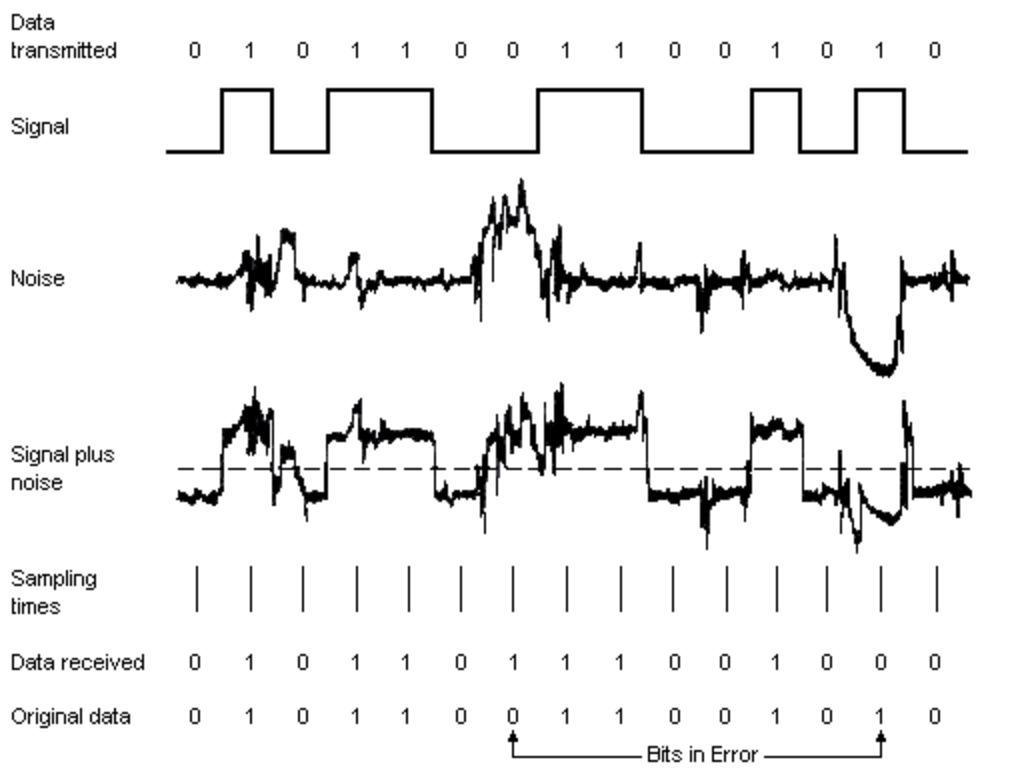
\includegraphics[scale = 0.4]{impulse_noise.png}
\end{center}

\item Block of information encoded into binary vector, called \textit{codeword}.
\vspace{3mm}

\item Error correcting codes check correctness of the codeword received.

\end{itemize}
\end{frame}


\begin{frame}
\frametitle{Linear Code}
\begin{itemize}
\item Set of codewords corresponding to a set of data vectors that can possible be transmitted is called the \textit{code}.
\vspace{4mm}

\item A code is said to be linear when adding two codewords of the code component-wise modulo-2 arithmetic results in a third codeword of the code.
\vspace{4mm}

\item A linear code $C$ can be represented by:
\begin{itemize}
\item codeword length $\ell$
\item message length $r$

\begin{center}
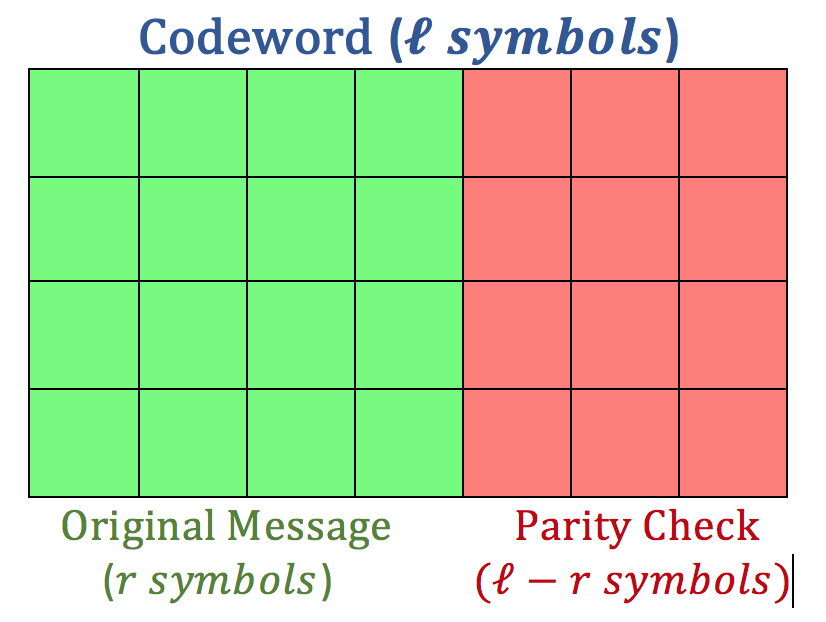
\includegraphics[scale = 0.3]{codeword.png}
\end{center}
\end{itemize}

\item To encode $r$ bits, we require $2^r$ unique codewords.

\end{itemize}
\end{frame}

%BCH Codes
\begin{frame}
\frametitle{BCH Codes}
\begin{itemize}
\item BCH codes form a class of cyclic error-correcting codes.
\vspace{4mm}

\item Linear code $C$ of length $n$ is a \textit{cyclic code} if it is invariant under a cyclic shift:
\[ \textbf{c} = (c_0, c_1, \hdots, c_{n-2}, c_{n-1} ) \in C \] if and only if 
\[ \tilde{\textbf{c}} = (c_{n-1}, c_0, c_1, \hdots, c_{n-2}) \in C, \] \cite{hall2003notes}.
\vspace{4mm}

\item For any two integers $t$ and $q$, a BCH code over $\mB{F}_2$ has length $\ell = 2^q -1$ and dimension $r = 2^q -1- tq$.
\vspace{4mm}

\item Any two codewords maintain a minimum Hamming distance of $2t + 1$.

\end{itemize}
\end{frame}


%CONNECTION TO CLASS
\begin{frame}
\frametitle{Connection to Randomized Methods} 
\begin{itemize} 
\item In class, we've discussed randomized methods including Subsampled Random Fourier and Hadamard Transforms (SRFT and SRHT, resp.)
\vspace{4mm}

\item Ubaru et al. \cite{ubaru2015low} propose using error correcting codes to find low rank approximations in a manner similar to SRF/HT.
\vspace{4mm}

\end{itemize}
\end{frame}

%SUBSAMPLE CODE MATRIX
\begin{frame}
\frametitle{Subsampled Code Matrix} 
\begin{itemize} 
\item Let $A$ be an $m \times n$ matrix with approximate rank $k$.
\vspace{3mm}

\item \textbf{Goal:} Construct a lower dimensional subsampling matrix $\Omega$ so that $Y = A \Omega$ provides ``good" approximation for range of $A$ while STILL preserving the geometry of $A$, i.e. distances are preserved.
\vspace{3mm}

\end{itemize}
\end{frame}

%P2
\begin{frame}
\frametitle{Subsampled Code Matrix} 
\begin{itemize} 
\item Let $A$ be an $m \times n$ matrix with approximate rank $k$.
\vspace{3mm}

\item \textbf{Goal:} Construct a lower dimensional subsampling matrix $\Omega$ so that $Y = A \Omega$ provides ``good" approximation for range of $A$ while STILL preserving the geometry of $A$, i.e. distances are preserved.
\vspace{3mm}

\item Choose the length of message $r \ge \lceil \log_2(n) \rceil$ and length of the code $\ell > k$, the target rank.
\vspace{3mm}

\end{itemize}
\end{frame}

%SUBSAMPLED
\begin{frame}
\frametitle{Subsampled Code Matrix} 
\begin{itemize} 
\item Form the Subsampling Code Matrix as:
\[ \Omega_{n \times \ell} = \sqrt{ \frac{2^r}{\ell}} D_{n \times n} S_{n \times 2^r} \Phi_{2^r \times \ell} \]
where

\begin{itemize}
\item $D$ is a random $n \times n$ diagonal matrix whose entries are independent random signs, i.e. random variables uniformly distributed on $\{ \pm 1 \}$.
\vspace{3mm}

\item $S$ is a uniformly random downsampler, an $n \times 2^r$ matrix whose $n$ rows are randomly selected from a $2^r \times 2^r$ identity matrix.
\vspace{3mm}

\item $\Phi$ is the $2^r \times \ell$ code matrix, generated using an $[ \ell, r ]$- linear coding scheme, with \textit{binary phase-shift keying} mapping and scaled by $2^{-r/2}$ such that all columns have unit norm.
\end{itemize}

\end{itemize}
\end{frame}

%SUBSAMPLED
\begin{frame}
\frametitle{Subsampled Code Matrix} 
\begin{itemize} 
\item Form the Subsampling Code Matrix as:
\[ \Omega_{n \times \ell} = \sqrt{ \frac{2^r}{\ell}} D_{n \times n} S_{n \times 2^r} \Phi_{2^r \times \ell} \]
where

\begin{itemize}
\item $D$ is a random $n \times n$ diagonal matrix whose entries are independent random signs, i.e. random variables uniformly distributed on $\{ \pm 1 \}$.
\vspace{3mm}

\item $S$ is a uniformly random downsampler, an $n \times 2^r$ matrix whose $n$ rows are randomly selected from a $2^r \times 2^r$ identity matrix.
\vspace{3mm}

\item $\Phi$ is the $2^r \times \ell$ code matrix, generated using an $[ \ell, r ]$- linear coding scheme, with \textit{binary phase-shift keying} mapping and scaled by $2^{-r/2}$ such that all columns have unit norm.
\vspace{3mm}

\end{itemize}

\item Binary Phase-Shift Keying (BPSK): Given a codeword $c \in C$, $c \mapsto \phi \in \mB{R}^{\ell}$ by assigning $1 \to \frac{-1}{\sqrt{2^r}}$ and $0 \to \frac{1}{\sqrt{2^r}}$.
\end{itemize}

\end{frame}

%PROPERTIES
\begin{frame}
\frametitle{Nice Properties of SCM} 
\begin{itemize} 
\item Define the \textit{dual} of a code as a code of length $\ell' = 2^q - 1 = \ell$, dimension $r' = tq$ and minimum distance at least $2^{q-1} - (t - 1)2^{q/2}$.
\vspace{3mm}

\item \textbf{Fact:} Any error correcting code matrix with dual distance > 4 (more than 2 error correcting ability) will satisfy the Johnson-Lindenstrauss Transform (JLT) property.
\vspace{3mm}

\begin{lemma}
Let $0< \epsilon, \delta < 1$ and $f$ be some function. It $\Omega \in \mB{R}^{n \times \ell}$ satisfies a JLT-($\epsilon, \delta, d$) with $\ell = O(k \log(k /\epsilon)/\epsilon^2. f(\delta))$, then for any orthonormal matrix $V \in \mB{R}^{n \times k}, n \ge k$ we have 
\[ \textbf{Pr}(|| V^T \Omega \Omega^TV - I||_2 \le \epsilon) \ge 1 - \delta. \]
\end{lemma}
\end{itemize}
\end{frame}

%PROPS 2
\begin{frame}
\frametitle{Nice Properties of SCM} 
\begin{itemize} 
\item Define the \textit{dual} of a code as a code of length $\ell' = 2^q - 1 = \ell$, dimension $r' = tq$ and minimum distance at least $2^{q-1} - (t - 1)2^{q/2}$.
\vspace{3mm}

\item \textbf{Fact:} Any error correcting code matrix with dual distance > 4 (more than 2 error correcting ability) will satisfy the Johnson-Lindenstrauss Transform (JLT) property.
\vspace{3mm}

\begin{lemma}
Let $0< \epsilon, \delta < 1$ and $f$ be some function. It $\Omega \in \mB{R}^{n \times \ell}$ satisfies a JLT-($\epsilon, \delta, d$) with $\ell = O(k \log(k /\epsilon)/\epsilon^2. f(\delta))$, then for any orthonormal matrix $V \in \mB{R}^{n \times k}, n \ge k$ we have 
\[ \textbf{Pr}(|| V^T \Omega \Omega^TV - I||_2 \le \epsilon) \ge 1 - \delta. \]
\end{lemma}

\vspace{3mm}
\item Above lemma shows that, any sampling matrix $\Omega$ satisfying JLT and having length $\ell = O(k \log(k/\epsilon) / \epsilon^2)$ satisfies the subspace embedding property.
\end{itemize}
\end{frame}

%PROPS 3
\begin{frame}
\frametitle{Nice Properties of SCM} 
\begin{itemize} 
\item Define the \textit{dual} of a code as a code of length $\ell' = 2^q - 1 = \ell$, dimension $r' = tq$ and minimum distance at least $2^{q-1} - (t - 1)2^{q/2}$.
\vspace{3mm}

\item \textbf{Fact:} Any error correcting code matrix with dual distance $> 4$ (more than 2 error correcting ability) will satisfy the Johnson-Lindenstrauss Transform (JLT) property.
\vspace{3mm}

\begin{lemma}
Let $0< \epsilon, \delta < 1$ and $f$ be some function. It $\Omega \in \mB{R}^{n \times \ell}$ satisfies a JLT-($\epsilon, \delta, d$) with $\ell = O(k \log(k /\epsilon)/\epsilon^2. f(\delta))$, then for any orthonormal matrix $V \in \mB{R}^{n \times k}, n \ge k$ we have 
\[ \textbf{Pr}(|| V^T \Omega \Omega^TV - I||_2 \le \epsilon) \ge 1 - \delta. \]
\end{lemma}
\vspace{3mm}

\item Above lemma shows that, any sampling matrix $\Omega$ satisfying JLT and having length $\ell = O(k \log(k/\epsilon) / \epsilon^2)$ satisfies the subspace embedding property.
\vspace{3mm}

\item Any SCM $\Omega$ with a dual distance $> 4$ will also satisfy the subspace embedding property. This shows SCM matrices can preserve the geometry of the top $k$-singular vectors of input matrix $A$.
\end{itemize}
\end{frame}
	
%Comparison and Results
\begin{frame}

\end{frame}

\begin{frame}[allowframebreaks]{Bibliography}
\bibliographystyle{abbrv}
\bibliography{presentation_bib}

\end{frame}


\end{document}